\subsection{Octree lineal}

Cada hoja se representa con el par $(c,\ell)$, donde $c$ es su \emph{location code}
y $\ell$ su nivel. Para una resolución $r$ fija, todos los códigos usan $3r$ bits:
una hoja de nivel $\ell<r$ tiene en cero sus $3(r-\ell)$ bits inferiores, de modo que
su código coincide con el de su celda de nivel $r$ de esquina mínima. Cada dígito
octal vale $x+2y+4z$, igual que en \texttt{encode}.

El octree se construye recursivamente desde el cubo $[0,1]^3$, visitando las ocho
hijas en orden $0,\dots,7$; así las hojas salen ya ordenadas por código (orden
Morton) y no hace falta ordenarlas después. Una celda de lado $a$ y centro $p$ no
puede contener la superficie $F=0$ si
\[
    |F(p)| > L\,\frac{\sqrt{3}}{2}\,a,
\]
donde $L$ es una constante de Lipschitz de $F$ en el cubo, porque ningún punto de la
celda está a más de una semidiagonal de su centro. En ese caso la celda se guarda
como una hoja grande; si no, se subdivide hasta el nivel $r$. Es el mismo test
(\texttt{canCross}) que usa Marching Cubes para encontrar las celdas de superficie,
así que toda celda de superficie es una hoja de nivel $r$, y también lo son las
cuatro celdas que comparten cada arista cortada (todas contienen el cero que hay
sobre la arista). Usamos $L=1.74$ para la esfera y $L=1.30$ para el toro, que
acotan $\|\nabla F\|$ en $[0,1]^3$ ($\sqrt{3}\approx 1.732$ y $\approx 1.289$).

El resultado es un arreglo ordenado, sin duplicados, cuyas hojas cubren todo el
cubo. Las regiones vacías quedan como pocas hojas grandes, pero el número de hojas
crece aproximadamente como $4^r$, igual que el área de la superficie medida en
celdas (cuadro~\ref{tab:obj2_hojas}).

\subsection{Verificación de existencia}

Ni Schrack ni Samet comprueban que el vecino calculado exista; es un paso aparte,
igual para ambos. Implementamos dos variantes que buscan el par exacto
$(c,\ell)$:
\begin{itemize}
  \item \textbf{Búsqueda binaria} (\texttt{hasLeaf}): \texttt{lower\_bound} sobre el
        arreglo ordenado, $O(\lg N)$ para $N$ hojas, sin memoria adicional.
  \item \textbf{Tabla hash} (\texttt{hasLeafHash}): un \texttt{unordered\_set} con
        clave (código, nivel), $O(1)$ esperado, a cambio de memoria extra y del
        tiempo de construir la tabla.
\end{itemize}
Encontrar una hoja de otro nivel con el mismo código no cuenta: el proyecto solo
trata vecinos de igual tamaño.

\subsection{Diseño experimental}

Las consultas son las que hace Marching Cubes al compartir vértices: para cada celda
de superficie, las vecinas por cara y por arista que necesita según las aristas que
corta la superficie (\texttt{buildQueries}). Su número crece con $r$ y depende de la
superficie. Antes de medir se verifica que, en todas las consultas, Schrack, Samet y
el oráculo (decodificar, sumar y codificar) devuelvan el mismo código y que la vecina
exista en ambas estructuras.

Para cada superficie, $r=4,\dots,10$, método y estructura hacemos cinco corridas.
En cada corrida se miden por separado tres tiempos: el cálculo de la dirección, la
verificación de existencia sobre las vecinas ya calculadas y la búsqueda completa
(ambas cosas en el mismo ciclo). Cuando hay pocas consultas, el lote se repite hasta
sumar al menos $2^{20}$ consultas por medición, y los tiempos se reportan en
nanosegundos por consulta. Se compiló con \texttt{g++ -O2} y se ejecutó en un hilo.

Las mediciones se hicieron en una laptop con Intel Core i7-13620H y 16~GB de RAM,
Windows~11 y g++~16.1, conectada a la corriente. Los datos crudos están en
\texttt{results/obj2.csv} y los promedios (con su desviación estándar) en
\texttt{results/obj2\_resumen.csv}.

\subsection{Resultados del objetivo 2}

\begin{table}[htbp]
\centering
\caption{Tamaño del octree, consultas de Marching Cubes y tiempo de construcción.}
\label{tab:obj2_hojas}
\begin{tabular}{lrrrrrr}
\toprule
Superficie & $r$ & Hojas & Celdas de superficie & Consultas & Octree (ms) & Tabla hash (ms) \\
\midrule
Esfera & 4  &      3\,032 &       584 &     1\,575 &     0.25 &      0.41 \\
Esfera & 5  &     14\,568 &     2\,408 &     6\,495 &     1.04 &      2.16 \\
Esfera & 6  &     61\,440 &     9\,488 &    25\,641 &     3.53 &      7.03 \\
Esfera & 7  &    249\,208 &    37\,856 &   102\,465 &    17.50 &     39.82 \\
Esfera & 8  &  1\,010\,192 &   151\,400 &   409\,845 &   246.57 &    268.95 \\
Esfera & 9  &  4\,053\,680 &   605\,264 & 1\,638\,567 &   290.21 &    964.86 \\
Esfera & 10 & 16\,202\,600 & 2\,421\,200 & 6\,554\,427 &  1\,349.49 &  3\,015.47 \\
\midrule
Toro & 4  &      3\,032 &       424 &     1\,166 &     1.71 &      0.33 \\
Toro & 5  &     15\,744 &     1\,840 &     4\,998 &     0.92 &      1.60 \\
Toro & 6  &     77\,680 &     7\,104 &    19\,402 &     4.78 &      9.70 \\
Toro & 7  &    378\,288 &    27\,720 &    75\,910 &    22.84 &     45.79 \\
Toro & 8  &  1\,910\,112 &   112\,040 &   306\,278 &   118.41 &    247.74 \\
Toro & 9  &  8\,032\,592 &   450\,760 & 1\,231\,236 &   533.73 &  1\,247.57 \\
Toro & 10 & 32\,507\,168 & 1\,798\,288 & 4\,914\,134 &  3\,083.83 & 12\,184.80 \\
\bottomrule
\end{tabular}
\end{table}

\begin{table}[htbp]
\centering
\caption{Tiempo medio por consulta (ns, promedio de 5 corridas). La columna de
dirección corresponde a las corridas con búsqueda binaria.}
\label{tab:obj2_tiempos}
\begin{tabular}{llrrrrr}
\toprule
 & & & \multicolumn{2}{c}{Binaria} & \multicolumn{2}{c}{Hash} \\
\cmidrule(lr){4-5}\cmidrule(lr){6-7}
Superficie, $r$ & Método & Dirección & Existencia & Total & Existencia & Total \\
\midrule
Esfera, 4  & Schrack &  27.82 &  78.72 & 146.42 & 11.57 &  37.38 \\
           & Samet   &  18.19 &  79.77 & 156.37 & 11.75 &  26.46 \\
           & Oráculo &  52.67 &  82.75 & 124.69 & 12.40 &  61.46 \\
Esfera, 7  & Schrack &  32.16 & 153.43 & 214.75 & 81.95 & 177.58 \\
           & Samet   &  42.28 & 166.80 & 274.44 & 78.58 & 158.52 \\
           & Oráculo &  91.94 & 165.89 & 237.41 & 62.77 & 209.33 \\
Esfera, 10 & Schrack &  28.78 & 170.77 & 233.41 & 77.94 & 146.48 \\
           & Samet   &  35.11 & 192.04 & 280.95 & 81.32 & 154.22 \\
           & Oráculo & 117.75 & 180.62 & 271.77 & 67.29 & 221.63 \\
\midrule
Toro, 4    & Schrack &  28.03 &  68.52 & 122.26 & 10.23 &  36.93 \\
           & Samet   &  17.27 &  65.95 & 114.30 & 10.43 &  28.02 \\
           & Oráculo &  51.82 &  69.04 & 107.03 & 10.25 &  57.67 \\
Toro, 7    & Schrack &  32.02 & 152.84 & 212.74 & 31.31 &  84.89 \\
           & Samet   &  42.44 & 152.51 & 222.71 & 31.40 &  88.24 \\
           & Oráculo &  80.50 & 149.94 & 220.21 & 30.10 & 138.41 \\
Toro, 10   & Schrack &  33.43 & 184.81 & 260.93 & 66.59 & 118.87 \\
           & Samet   &  32.63 & 185.18 & 261.11 & 60.00 & 119.07 \\
           & Oráculo & 108.29 & 179.01 & 253.39 & 56.44 & 201.00 \\
\bottomrule
\end{tabular}
\end{table}

\begin{figure}[htbp]
\centering
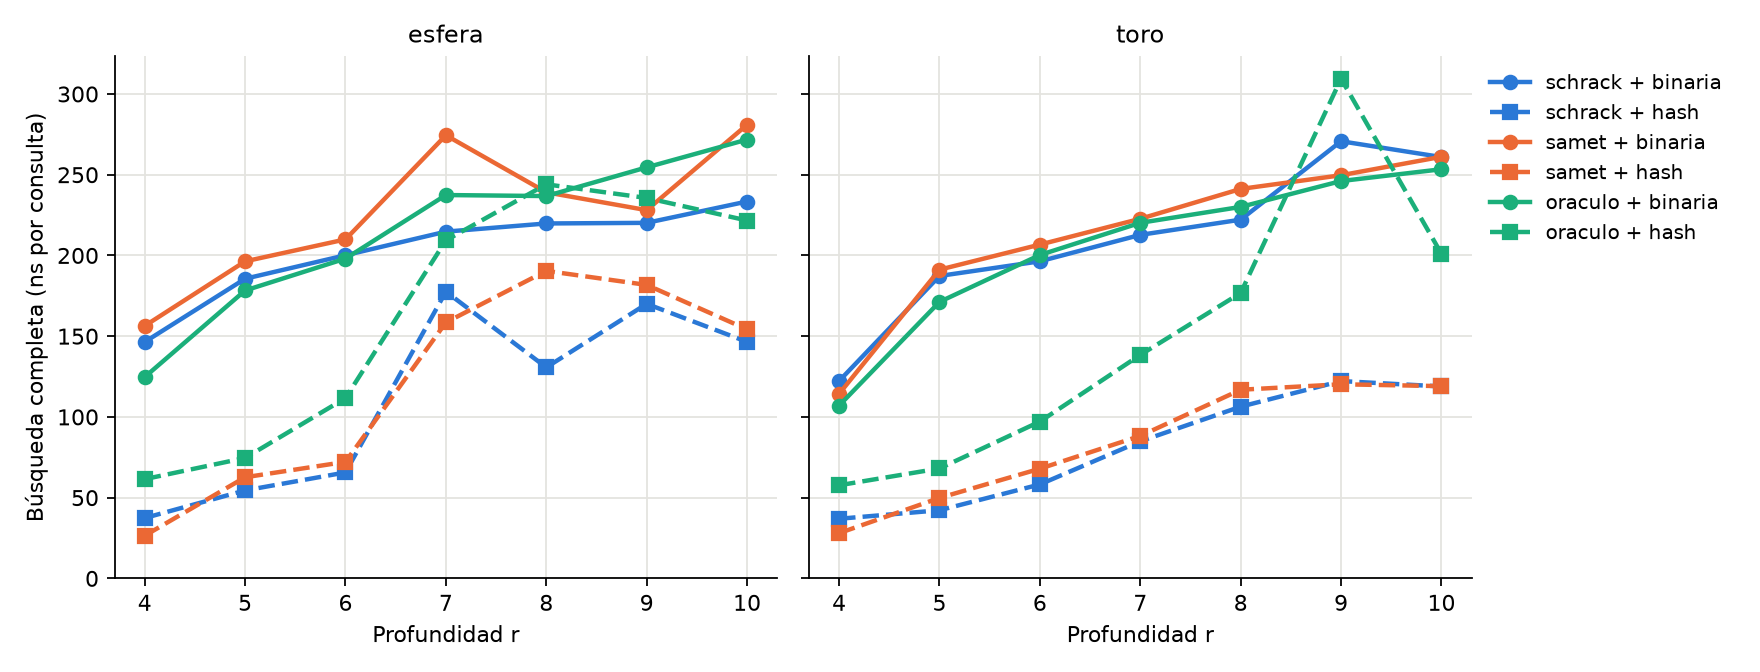
\includegraphics[width=\linewidth]{results/obj2_total.png}
\caption{Búsqueda completa (dirección más existencia) por consulta de Marching Cubes.}
\label{fig:obj2_total}
\end{figure}

\begin{figure}[htbp]
\centering
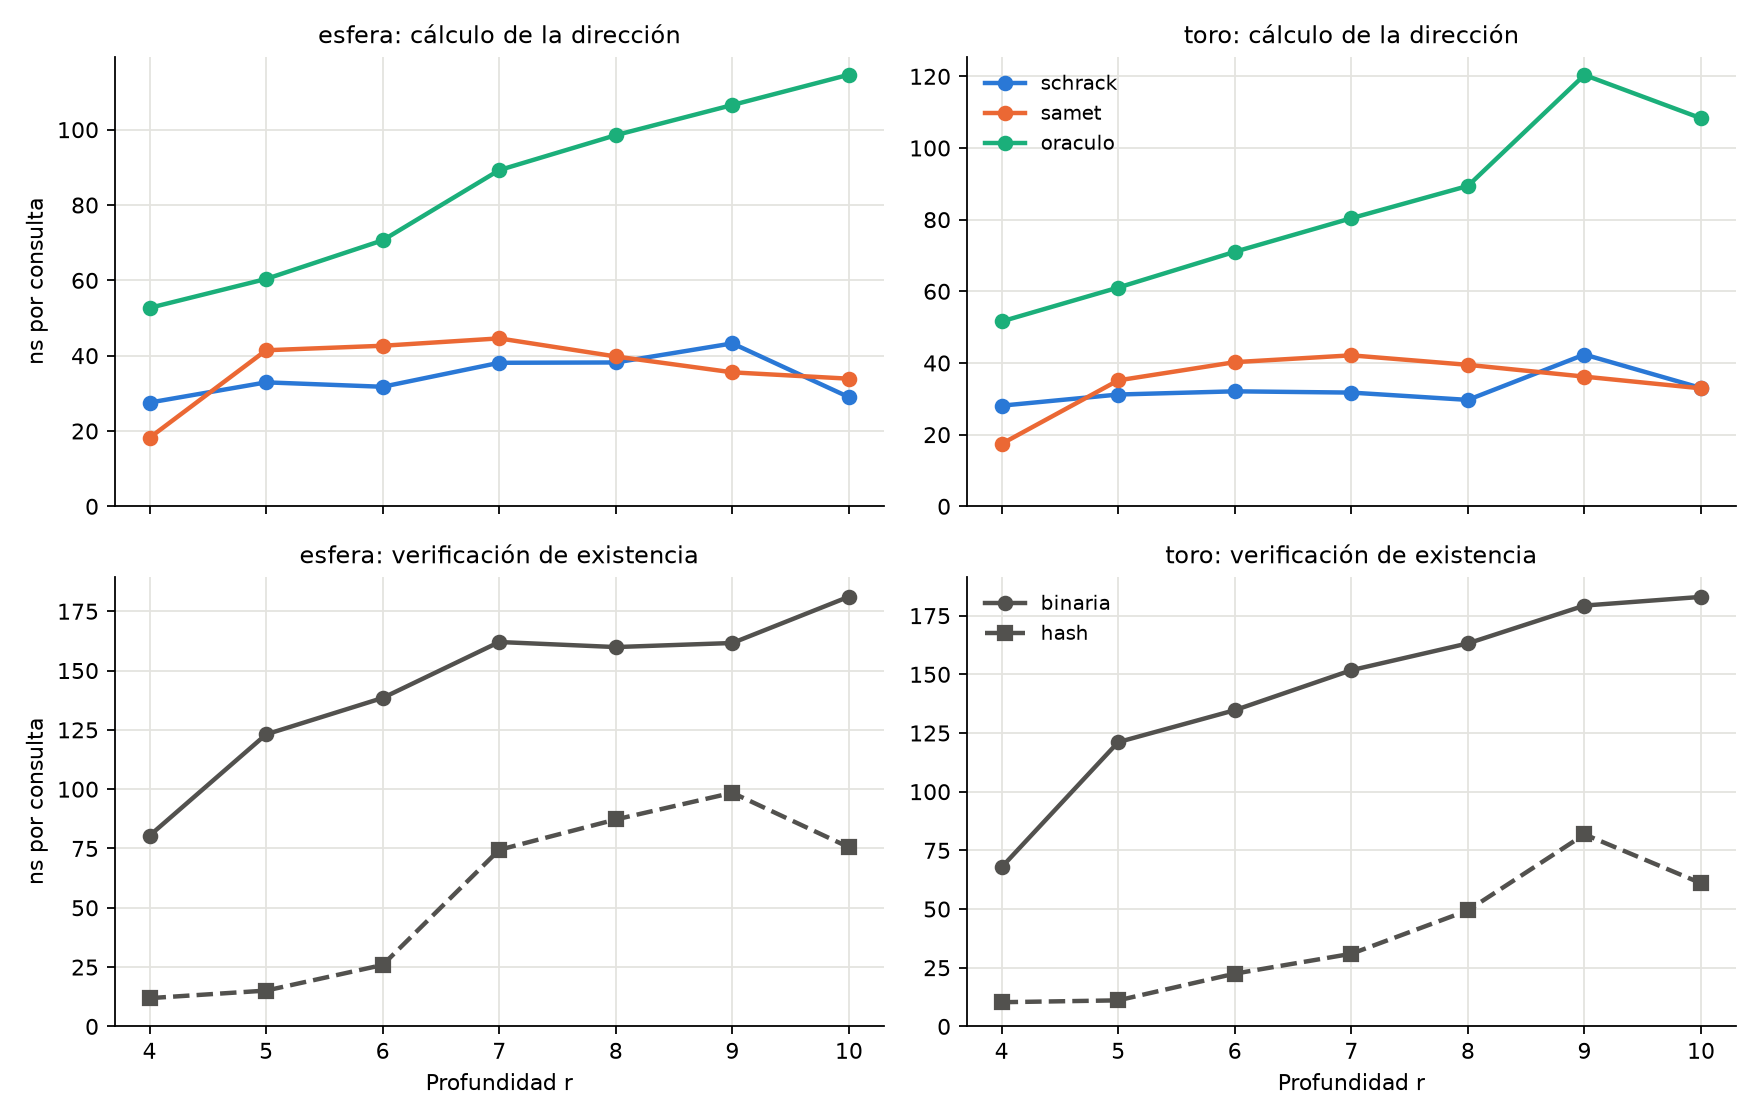
\includegraphics[width=\linewidth]{results/obj2_componentes.png}
\caption{Cálculo de la dirección por método y verificación de existencia por
estructura, medidos por separado.}
\label{fig:obj2_componentes}
\end{figure}

\paragraph{Tamaño.} Entre $r=9$ y $r=10$ el número de hojas se multiplica por
$4.0$ en ambas superficies (cuadro~\ref{tab:obj2_hojas}). Con $r=10$ el toro llega a
32.5 millones de hojas; el arreglo ocupa unos 520~MB y la tabla hash bastante más.

\paragraph{Cálculo de la dirección.} En las consultas de Marching Cubes, Schrack
no crece con $r$: en 11 de las 14 configuraciones está entre 28 y 34~ns, con picos
de 42 a 52~ns en las otras tres. Samet da 17--18~ns para $r=4$ y 33--43~ns para
$r\ge 5$ (corridas con binaria). El oráculo, que
recorre los $r$ dígitos al decodificar y codificar, crece de 52 a 118~ns
(figura~\ref{fig:obj2_componentes}). Es decir, en estas consultas la reflexión de
dígitos cuesta lo mismo que Schrack: los vecinos que pide Marching Cubes están a
una celda de distancia y casi siempre comparten un ancestro cercano, así que Samet
refleja pocos dígitos. Es el obstáculo previsto en la propuesta; la ventaja de
Schrack en el peor caso se estudia en el objetivo~1.

\paragraph{Verificación de existencia.} Es la parte dominante. Con búsqueda
binaria pasa de 66--83~ns en $r=4$ a 171--192~ns en $r=10$; con $r=10$ representa
alrededor del 85\,\% de la suma de dirección más existencia, con Schrack y con
Samet. La tabla hash es mucho más rápida en $r$ pequeño (10--12~ns), pero tampoco es
constante en la práctica: sube a 56--81~ns en $r=10$, cuando la tabla ya no cabe en
la caché y cada consulta es un acceso aleatorio a memoria.

\paragraph{Búsqueda completa.} Con $r=10$ y los métodos de Schrack o Samet, la
búsqueda completa cuesta 233--281~ns con binaria y 119--154~ns con hash
(cuadro~\ref{tab:obj2_tiempos}). Entre Schrack y
Samet no hay una diferencia consistente: en el toro con $r=10$ dan 260.93 y
261.11~ns con binaria. Además, el total medido es mayor que la suma de dirección y
existencia medidas por separado (por ejemplo, $28.78+170.77=199.55$ frente a
233.41~ns en la esfera con Schrack y binaria). Al medir la existencia sola, las
vecinas se leen de un arreglo y el procesador puede adelantar varias búsquedas a la
vez; dentro del ciclo completo cada búsqueda depende del cálculo de su dirección.
Por eso reportamos los tres tiempos.

\paragraph{Costo de construir la tabla hash.} Con $r=10$, construir la tabla hash
tarda 2.2 veces lo que tarda construir el octree en la esfera (3.0~s) y 4.0 veces en
el toro (12.2~s). Con Schrack, ahorra 86.9~ns por consulta en la esfera y 142.1~ns en el
toro; con las consultas de una sola pasada de Marching Cubes son 0.57~s y 0.70~s.
Para recuperar el costo de construirla harían falta unas 5 pasadas en la esfera y
unas 17 en el toro. Para una sola reconstrucción de la malla conviene la búsqueda
binaria; la tabla solo compensa si el mismo octree se consulta muchas veces.

\paragraph{Variabilidad.} En 67 de las 84 configuraciones la desviación estándar del
total es de 15~ns o menos (mediana 5.3~ns), pero hay picos aislados. Por ejemplo, una de las cinco
corridas de oráculo con hash en el toro con $r=9$ tardó 535.91~ns, lo que eleva su
promedio a 309.43~ns. Los promedios de \texttt{obj2\_resumen.csv} incluyen esas
corridas; la desviación estándar de cada configuración está en el mismo archivo.
